% Koma-Script Report, verkleinerte Überschriftenstile, Linie unter der Kopfzeile
\documentclass[ 11pt
				,ngerman
				,headsepline
				,headings=small
				,numbers=noenddot %kein Punkt hinter letzter Gliederungsziffer Abschnitt 2.1 statt 2.1.
				,draft=false
				,BCOR=0mm %Wert für Bindekorrektur kann hier eingestellt werden
				,DIV=12
				,captions=tableheading
				,paper=a4
				,abstracton
                ]{scrreprt}

%%%%%%%%%%%%%%%%%%%%%%%%%%%%%%%%%%%%%%%%%%%%%%%%%%%%%%%%%%%%%%%%%%%%%%%%%%%%%%%
% Basispakete
%%%%%%%%%%%%%%%%%%%%%%%%%%%%%%%%%%%%%%%%%%%%%%%%%%%%%%%%%%%%%%%%%%%%%%%%%%%%%%%
\usepackage[utf8]{inputenc} 
\usepackage[ngerman]{babel} %Anpassungen an nicht-englische Sprachen
\usepackage{ifpdf} 
%%%%%%%%%%%%%%%%%%%%%%%%%%%%%%%%%%%%%%%%%%%%%%%%%%%%%%%%%%%%%%%%%%%%%%%%%%%%%%%
                
%%%%%%%%%%%%%%%%%%%%%%%%%%%%%%%%%%%%%%%%%%%%%%%%%%%%%%%%%%%%%%%%%%%%%%%%%%%%%%%
% Schriftarten, Schriftschnitte etc.
%%%%%%%%%%%%%%%%%%%%%%%%%%%%%%%%%%%%%%%%%%%%%%%%%%%%%%%%%%%%%%%%%%%%%%%%%%%%%%%
\usepackage{fourier} %PDF-kompatible Schriftfamilie "Utopia", Freierhältliches Look-alike: Heuristica
\makeatletter % Warnungen zu Schriftartersetzungen unterdrücken
  \let\@font@info\@gobble
  \let\@font@warning\@gobble
\makeatother

\usepackage[official]{eurosym} % Eurosymbol
\DeclareUnicodeCharacter{20AC}{\euro} % Standard-Euro-Symbol wird durch qualitativ hochwertiges Eurosymbol ersetzt

\renewcommand{\caplabelfont}{\bfseries} % Fettdruck für Abb. und Tab.

\usepackage{color}
\definecolor{ercred}{RGB}{229,48,39}

\usepackage{setspace} % Einstellen von Zeilenabständen
\onehalfspacing % Anderthalbzeiliger Satz

\setlength\parskip{\medskipamount} % Abstand zwischen zwei Absätzen
\setlength\parindent{0pt} % Keine Einrückung in der ersten Zeile eines Absatz

\AtBeginDocument{
  \renewcommand{\labelitemi}{\(\triangleright\)} %definiert die Art der Aufzählungszeichen
  \renewcommand{\labelitemii}{\(\bullet\)}}
%%%%%%%%%%%%%%%%%%%%%%%%%%%%%%%%%%%%%%%%%%%%%%%%%%%%%%%%%%%%%%%%%%%%%%%%%%%%%%%

%%%%%%%%%%%%%%%%%%%%%%%%%%%%%%%%%%%%%%%%%%%%%%%%%%%%%%%%%%%%%%%%%%%%%%%%%%%%%%%
% Layout der Seiten
%%%%%%%%%%%%%%%%%%%%%%%%%%%%%%%%%%%%%%%%%%%%%%%%%%%%%%%%%%%%%%%%%%%%%%%%%%%%%%%
\usepackage{fancyhdr} %Einstellung der Kopfzeile, Chaptermark auskommentieren wenn ein Stil one Kapitel gewählt wird (z.B. scrartcl)
\pagestyle{fancy} % Notwendig um die nächsten beiden Neudefinitionen vorzunehmen
\renewcommand{\sectionmark}[1]{\normalsize\markright{\thesection{} #1}{}}
\renewcommand{\chaptermark}[1]{\normalsize\markboth{#1}{}}
\interfootnotelinepenalty=10000 % Fußnoten nicht über zwei Seiten verteilen
%%%%%%%%%%%%%%%%%%%%%%%%%%%%%%%%%%%%%%%%%%%%%%%%%%%%%%%%%%%%%%%%%%%%%%%%%%%%%%%

%%%%%%%%%%%%%%%%%%%%%%%%%%%%%%%%%%%%%%%%%%%%%%%%%%%%%%%%%%%%%%%%%%%%%%%%%%%%%%%
% Tabellen
%%%%%%%%%%%%%%%%%%%%%%%%%%%%%%%%%%%%%%%%%%%%%%%%%%%%%%%%%%%%%%%%%%%%%%%%%%%%%%%
\usepackage{longtable}
\usepackage{multirow}
\usepackage{booktabs} % erzeugt besser aussehende Tabellen, horizontale Linien mit \toprule, \midrule, \bottomrule
\usepackage[point]{rccol} %Richtet Zahlen in Tabellen nach Dezimalkomma aus, im Output wird ein Dezimalpunkt verwendet
%%%%%%%%%%%%%%%%%%%%%%%%%%%%%%%%%%%%%%%%%%%%%%%%%%%%%%%%%%%%%%%%%%%%%%%%%%%%%%%

%%%%%%%%%%%%%%%%%%%%%%%%%%%%%%%%%%%%%%%%%%%%%%%%%%%%%%%%%%%%%%%%%%%%%%%%%%%%%%%
% Abbildungen
%%%%%%%%%%%%%%%%%%%%%%%%%%%%%%%%%%%%%%%%%%%%%%%%%%%%%%%%%%%%%%%%%%%%%%%%%%%%%%%
\usepackage{subfigure}
\usepackage{float}
%%%%%%%%%%%%%%%%%%%%%%%%%%%%%%%%%%%%%%%%%%%%%%%%%%%%%%%%%%%%%%%%%%%%%%%%%%%%%%%

%%%%%%%%%%%%%%%%%%%%%%%%%%%%%%%%%%%%%%%%%%%%%%%%%%%%%%%%%%%%%%%%%%%%%%%%%%%%%%%
% Mathematik
%%%%%%%%%%%%%%%%%%%%%%%%%%%%%%%%%%%%%%%%%%%%%%%%%%%%%%%%%%%%%%%%%%%%%%%%%%%%%%%
\usepackage{amsmath}
\usepackage{amssymb}
\usepackage{array}
\usepackage[cdot,thickqspace,squaren,textstyle]{SIunits} % SI-Einheiten sind als Befehle verfügbar
%%%%%%%%%%%%%%%%%%%%%%%%%%%%%%%%%%%%%%%%%%%%%%%%%%%%%%%%%%%%%%%%%%%%%%%%%%%%%%%

%%%%%%%%%%%%%%%%%%%%%%%%%%%%%%%%%%%%%%%%%%%%%%%%%%%%%%%%%%%%%%%%%%%%%%%%%%%%%%%
% Referenzen und Zitate
%%%%%%%%%%%%%%%%%%%%%%%%%%%%%%%%%%%%%%%%%%%%%%%%%%%%%%%%%%%%%%%%%%%%%%%%%%%%%%%
\usepackage{varioref}
\usepackage[square]{natbib}
\usepackage{bibunits}
%%%%%%%%%%%%%%%%%%%%%%%%%%%%%%%%%%%%%%%%%%%%%%%%%%%%%%%%%%%%%%%%%%%%%%%%%%%%%%%


%%%%%%%%%%%%%%%%%%%%%%%%%%%%%%%%%%%%%%%%%%%%%%%%%%%%%%%%%%%%%%%%%%%%%%%%%%%%%%%
% PDF-Einstellungen
%%%%%%%%%%%%%%%%%%%%%%%%%%%%%%%%%%%%%%%%%%%%%%%%%%%%%%%%%%%%%%%%%%%%%%%%%%%%%%%
\ifpdf
	%we are running PDFLaTeX
	\usepackage[pdftex]{graphicx} 
	\pdfimageresolution=100
	\pdfminorversion=7
	\pdfcompresslevel=9
	\usepackage[pdftex,
		urlcolor=blue,
		linktocpage,
		colorlinks=true,
		linkcolor=black,
		citecolor=black,
		pdfview=FitH,
		pdfstartview=FitH,
		plainpages=false]{hyperref}
	\hypersetup{
		pdfauthor={Deine Name},
        pdftitle={Titel des Berichts},
        pdfsubject={},
        pdfkeywords={Mehrere aussagekräftige Schlagwörter},
        pdfproducer={LaTeX with hyperref},
        pdfcreator={pdflatex}}
    \usepackage[figure,figure*]{hypcap}
\else
	%DVI or PS output
	\usepackage{graphicx} 
\fi
%%%%%%%%%%%%%%%%%%%%%%%%%%%%%%%%%%%%%%%%%%%%%%%%%%%%%%%%%%%%%%%%%%%%%%%%%%%%%%%

\begin{document}
\pagestyle{empty}
\newcounter{Hilfszaehler}

%%%%%%%%%%%%%%%%%%%%%%%%%%%%%%%%%%%%%%%%%%%%%%%%%%%%%%%%%%%%%%%%%%%%%%%%%%%%%%%
% HIER GEHT ES WIRKLICH LOS 
%%%%%%%%%%%%%%%%%%%%%%%%%%%%%%%%%%%%%%%%%%%%%%%%%%%%%%%%%%%%%%%%%%%%%%%%%%%%%%%

% Setup der normalen Seiten
%%%%%%%%%%%%%%%%%%%%%%%%%%%%%%%%%%%%%%%%%%%%%%%%%%%%%%%%%%%%%%%%%%%%%%%%%%%%%%%
\newpage
\pagenumbering{arabic}
\pagestyle{fancy}\lhead{\leftmark}\chead{}\rhead{\rightmark}
\rhead{\rightmark}
\lhead{\leftmark}
%%%%%%%%%%%%%%%%%%%%%%%%%%%%%%%%%%%%%%%%%%%%%%%%%%%%%%%%%%%%%%%%%%%%%%%%%%%%%%%

\chapter{Teil1}
\label{cha:Teil1}
\section{Motivation}
\label{sec:Motivation}

\begin{normalsize}
\begin{LARGE}

Die Bereitstellung von Wärme und elektrischer Energie beeinflusst immer stärker das Klima. Nach wie vor wird zumeist die Energie fossiler Energieträger genutzt, um den Bedarf zu decken. Um den Einfluss unseres Energiebedarfs auf das Klima zu reduzieren, wurden in den vergangenen Jahrzehnten verschiedene Versuche unternommen die Energiebereitstellung auf nachhaltige Quellen umzustellen. In diesem Zusammenhang ergibt sich das Ziel die Anreicherung von in der Erde gespeichertem Kohlenstoff als Kohlenstoffdioxid oder in Form anderer klimabeeinflussender Gase, wie zum Beispiel Methan, in der Atmosphäre zu verhindern. 
Die am meisten genutzten Quellen sind hierbei die Wasserkraft, Wind und Sonne. Wobei die Nutzbarkeit aller drei genannten Quellen stark von den geologischen, klimatischen und geographischen Bedingungen der jeweiligen Region abhängen und in den meisten Regionen starken Leistungsschwankungen unterliegen, sodass sich Problematiken in der Speicherung der Energie ergeben. Des Weiteren ist die Nutzung der genannten Quellen oft Kostenintensiver als das Verbrennen fossiler Ressourcen und der kostenintensive Umbau beziehungsweise Neubau einer entsprechenden Infrastruktur ist nötig. Dies hat in Deutschland in den vergangenen Jahren zu einem erheblichen Anstieg der Stromgestehungskosten und der Endenergiepreise geführt. Deshalb haben in den letzten Jahren die Bemühungen verschiedener Seiten zugenommen den Energieverbrauch zu senken. Für Privat genutzte Häuser und Wohnungen geschieht das in Deutschland vor allem über die "Verordnung über energiesparenden Wärmeschutz und energiesparende Analgentechnik bei Gebäuden", kurz EnEV,  von staatlicher Seite. 

%Stromgestehungskosten checken
Ziel ist es durch eine gute Isolierung den
 Wärmeverlust der Häuser zu reduzieren. 


Um entsprechende Gebäude mit 

ausreichend Frischluft zu versorgen,
 wird die Luft mittels eines Lüftungs
systems ausgetauscht und durch den Einsatz von Wärme
übertragern der Wärme-verlust über die ausgetauschte Luft reduziert. 
% Quelle EnEV (11)

Eine Konsequenz dieses Vorgehens in gemäßigten und kalten Klimaregionen ist ein Austrocknen der Raumluft. Die kalte Außenluft weißt einen geringen absoluten Wassergehalt auf. Beim Erhitzen im Wärmeübertrager stellt sich so eine sehr geringe relative Feuchte ein. 

Da an Wohngebäude und Bürogebäude oft hohe Anforderungen bezüglich der Luftqualität gestellt werden, ist es in vielen Fällen Sinnvoll die Luft auf eine Feuchtegehalt zu Konditionieren, der von den Menschen als angenehm empfunden wird und keine negativen Auswirkungen auf ihren Gesundheitszustand oder ihre Leistungsfähigkeit hat. Eine detaillierte Zusammenfassung über die Auswirkungen zu trockener Luft liefert 
%Quelle einfügen Energetische Bewertung von Wohnungslüftungsgeräten mit Feuchterückgewinnung (12)

In feucht warmen Klimazonen tritt oft ein gegenteiliger Effekt auf. Die feucht warme Zuluft wird abgekühlt und gewinnt so an relativer Feuchte. Dies kann dazu führen, dass Feuchteschäden an Bauteilen oder am Interieur des Gebäudes entstehen oder es zur Bildung von Schimmel kommt. Entsprechend ist hier in vielen Fällen eine Trocknung der zugeführten Luft notwendig. 
%[Zhang HB and Hiroshi Y. Analysis of indoor humidity environment in Chinese residential buildings. Build Environ 2010; 45(10): 2132–2140]

In Sonderfällen ist es möglich,


 dass bestimmte Raumklima-bedingungen 
 eingehalten werden müssen. 


Zum Beispiel bestimmte Lagerbedingungen oder 
Rahmenbedingungen für Produktionsabläufe oder Forschungs-prozesse. 
Das Trocknen beziehungsweise Befeuchten der Luft kostet viel Energie.
 
 
 Bei einem Luftbefeuchter muss hierzu die 
 Verdampfungsenthalpie des Wassers überwunden werden, 
 eine Beschreibung des Energieverbrauchs 
 von klassisch zur Trocknung von Luft eingesetzten 
 Sorptionstrocknern findet sich beispielsweise in 
 %Quelle evtl genauer darstellen, wenn ich später einen rechenfaktor auf dieser größe einführen möchte. 

Enthalpietauscher stellen eine Möglichkeit da,
 diese Energieaufwände zu reduzieren. 

\section{Enthalpieübertrager}
\label{Enthalpieübertrager}

Aus dem Stand der Technik sind vor allem Rotationsenthalpieübertrager und membranbasierte Enthalpieübertrager bekannt. Beide Systeme übertragen neben Wärme auch Feuchte von einem feuchten auf einen trockenen Luftstrom. Die Triebkraft in beiden Systemen ist das chemische Potenzial, das ausgeglichen wird. 

\begin{figure}
	\centering
	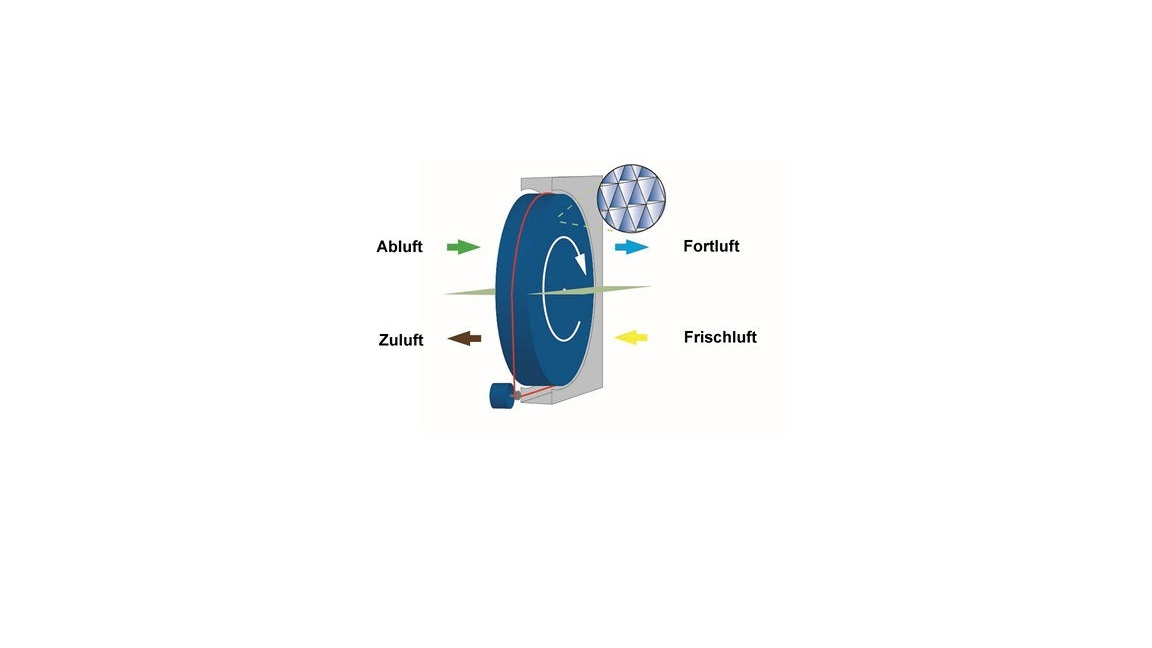
\includegraphics[width=10]{Pictures/Rotationswärmeübertrager.jpg}
	\includegraphics[width=10]{Pictures/Enthalpieübertrager.jpg}
\end{figure}

Rotationsübertrager weisen einen rotierende thermische Masse auf, die sich jeweils mit einem Teil der Masse im Zuluftstrom und mit einem anderen Teil der Masse im Abluftstrom befindet. Durch die Rotation kann die Masse thermische Energie in einem Luftstrom aufnehmen und nach dem Weiterrotieren im anderen Luftstrom abgeben. Analog funktioniert die Übertragung der Feuchte, wobei die Feuchte entweder von einem Sorptionsmaterial aufgenommen und wieder abgegeben wird oder in einem Luftstrom an der Masse kondensiert und im anderen Luftstrom wieder verdampft. Rotationsübertrager befinden sich bereits seit einigen Jahren kommerziell im Einsatz und wurden bereits entsprechend detailliert untersucht. %Quelle Bsp Performance comparisons of desiccant wheels for air dehumidification and enthalpy recovery
Membranbasierte Enthalpieübertrager sind erst seit wenigen Jahren kommerziell im Einsatz, sodass es bisher nur wenigen Untersuchungen zu ihnen exestieren. Die Wärme wird dann über die Membran von einem Luftstrom über an den anderen übertragen. Analog zum übertragenen Wärmestrom wird die Feuchte übertragen, das heißt Wasser wird vom Membranmaterial absorbiert, diffundiert durch die Membran und desorbiert auf der anderen Seite in den Luftstrom. Die Geometrien die Dabei für den Enthalpieübertrager verwendet werden, entsprechen denen, die bei klassischen Wärmeübertragern zum Einsatz kommen. In kommerziellen Anwendungen kommen Kreuzstromübertrager und Kreuzgegenstromübertrager zur Anwendung, wobei auch Gegenstromübertrager und "hollow fibre" Module mögliche Bauform darstellen. Kreuzstromübertrager sind im Vergleich zu Gegenstromübertragern Kostengünstig herstellbar und benötigen nur geringen Bauraum, daher sind sie die bisher häufigste Bauform bei Enthalpietauschern. Gegenstromübertrager haben im Gegensatz dazu einen hohen Wirkungsgrad. Deshalb hält vor allem eine Mischform aus beidem, der Kreuzgegenstromübertrager, immer stärker Einzug in die kommerzielle Nutzung. Hollow fibre Module ermöglichen hohe Übertragungsflächen bei kleinem Bauraum und somit hohe Übertragungsraten für Wärme und Feuchte. Nachteilig ist jedoch ein sehr hoher Druckverlust in den Modulen, der bisher verhindert hat, das diese Bauform sich in kommerziellen Anwendungen durchsetzen konnte. 

%\begin{figure}
%	\centering
%	\includegraphics[width=10]{pictures/Vergleich_Geometirie.jpg}
%	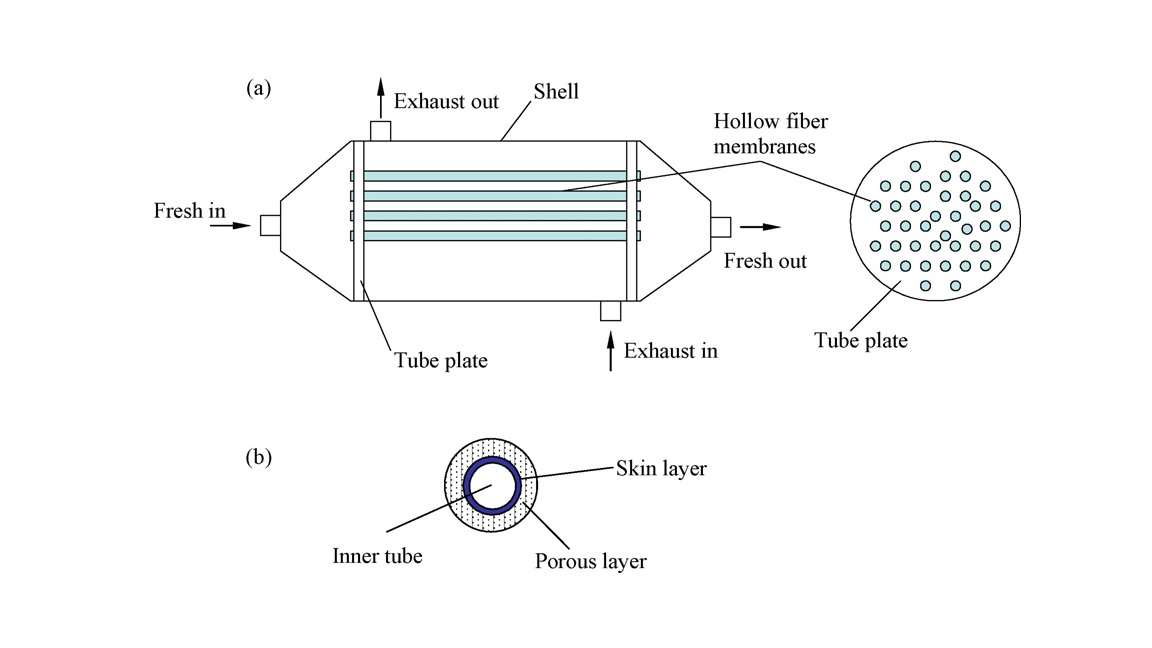
\includegraphics[width=10]{pictures/hollow_fibre.jpg}
%\end{figure}

Ein Vergleich zwischen Rotationsübertragern und membranbasierten Enthalpietauschern fällt je nach Untersuchung unterschiedlich aus. Grundlegend haben je doch membranbasierte Enthalpietauscher den Vorteil, dass sie keine beweglichen (rotierenden) Teile haben, was sie weniger verschleißanfällig macht und die Geräuschemissionen senkt. Außerdem muss keine Energie zum Antrieb eines Rotors aufgewendet werden. In den meisten Fällen besitzen membranbasierte Enthalpietauscher den höheren Wirkungsgrad. Nachteilig ist, dass sie nicht Regelbar sind. Bei besonders feucht warmen Tagen ist es daher möglich, das ein Enthalpieübertrager zur Feuchterückgewinnung der Zuluft zu viel Wasser zuführt, dies kann nur durch einen Bypass, eine Trockner oder einen Austausch des Enthalpieübertragers durch einen Wärmeübertrager für die entsprechende Jahreszeit verhindert werden. Außerdem können die membranbasierten Übertrager bei zu kalten Temperaturen zufrieren und müssen daher in einigen Klimazonen mit Vorheizern ausgestattet werden. Derzeit beherrschen Rotationsübertrager vor allem den Markt bei großen Anwendungsfällen während Enthalpieübertrager vor allem für Wohnungs- und Einzelraumlüftungen genutzt werden.  


\section{Membran}

Grundsätzlich lassen sich Membranen in dichte und poröse Membranen unterteilen. Poröse Membranen weisen Poren auf, die größer sind als die Partikel, die durch die Membran übertragen werden. Daher findet der Stofftransport aufgrund von.... statt. Dichte Membranen weisen hingegen Poren auf, die kleiner sind. Daher kann kein Stoffübertrag mehr auf Grund von ... stattfinden. Ein Stofftransport findet entsprechend nur noch auf Grund von Diffusion statt. Dies führt in den meisten Fällen zu einer deutlich erhöhten Selektivität und einer geringeren Permeabilität im Vergleich zu porösen Membranen. Da im vorliegenden Anwendungsfall Wasserdampf als Permeat die Membran passieren soll und kleine gasförmige Moleküle der Luft, wie Stickstoff zurückgehalten werden sollen, ist eine Dichte Membran sinnvoll, da nur so eine ausreichende Selektivität gegenüber den gasförmigen Komponenten gewährleistet werden kann. Um dennoch eine möglichst hohe Permeabilität gegenüber Wasserdampf zu gewährleisten ist es zielführend eine möglichst dünne Membran zu verwenden. Um die dünnnen dichten Membranen mechanische zu stabilisieren wird die dichte Membran in einigen Fällen durch eine poröse Membran gestützt, diese hat kaum negative Auswirkungen auf die Permeabilität, die Transportgeschwindigkeiten in porösen Membranen wesentlichen höher sind als in dichten Membranen. Gleichzeitig kann eine günstige Geometrie der Spacermaterialien und der porösen Membranen zu besseren Wärmeübergangskoeffizienten und Sorptionseigenschaften an der Membranoberfläche auf Grund von vorteilhaften Strömungseigenschaften führen. %auf wasseraffinität eingehen
\begin{figure}
	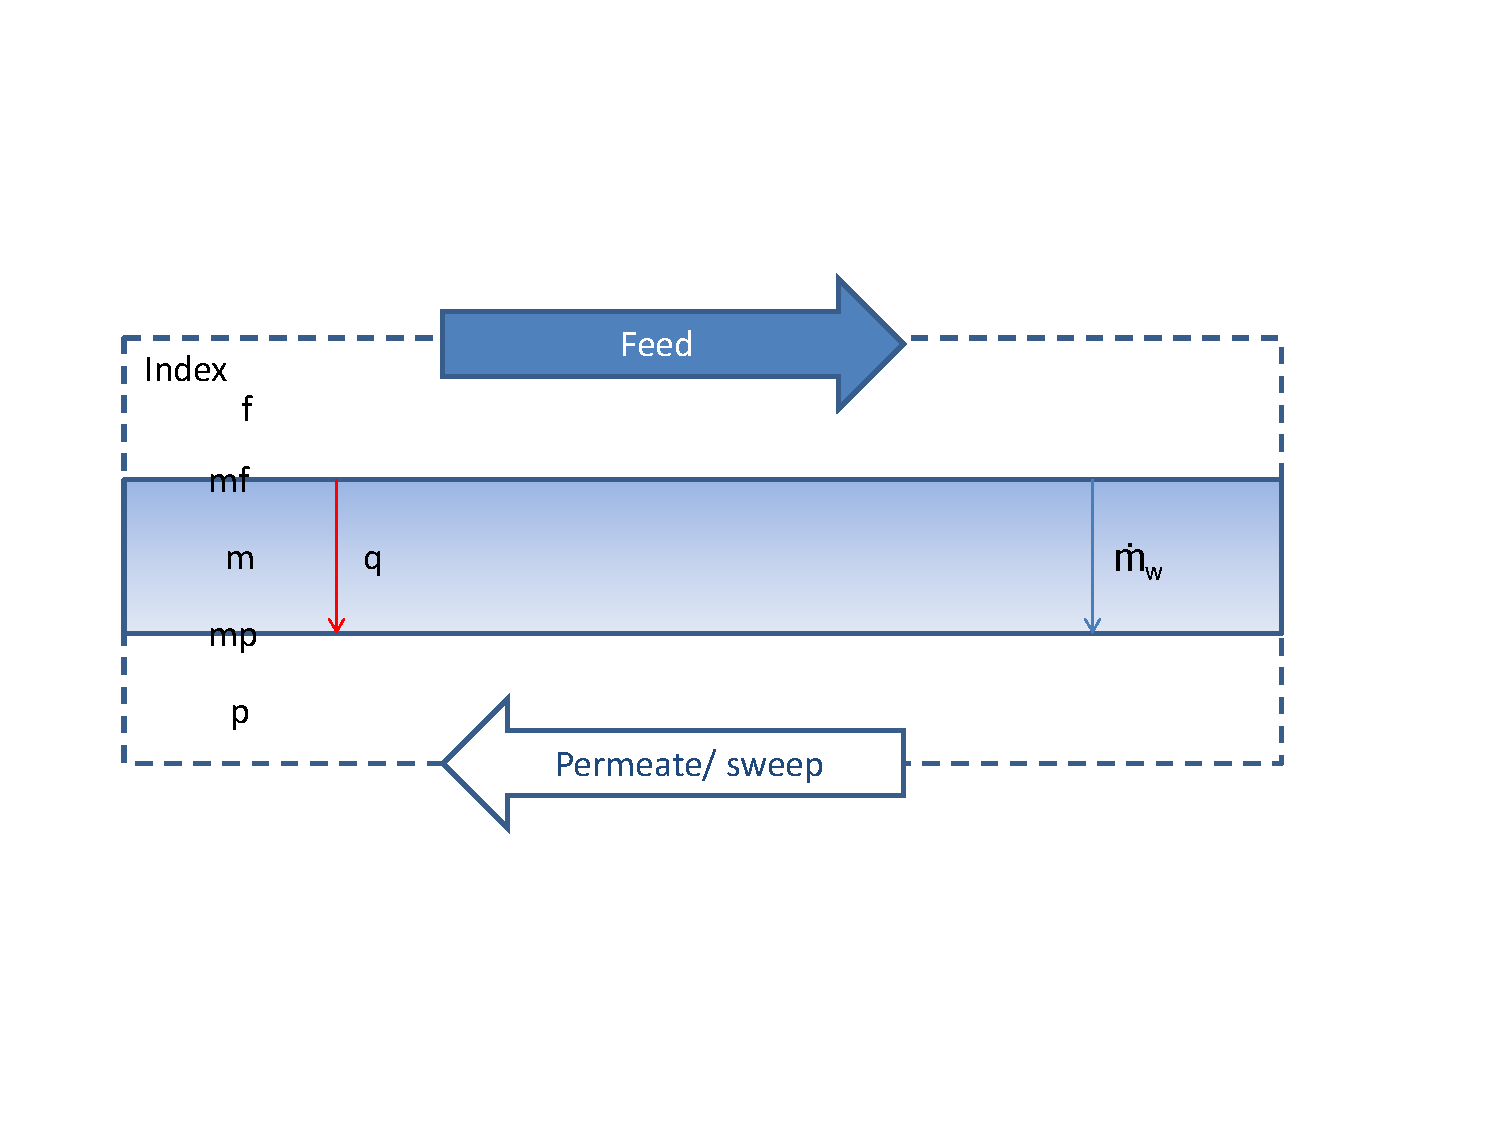
\includegraphics[width=10]{Membran}
\end{figure}

In Enthalpieübertragern werden derzeit Membranen aus Papier oder Polymeren eingesetzt. Die technische Weiterentwicklung der Polymermembranen über die letzten Jahre hat dazu geführt, das mittlerweile fast ausschließlich Polymermembranen zu Einsatz kommen, da diese deutlich höhere Permeabilitäten aufweisen. 

Der Transport des Wasser von einem Luftstrom in den anderen Luftstrom durch die Membran lässt sich in 3 Phasen einteilen. Zuerst wird das Wasser auf einer Seite von der Membran Absorbiert, dann diffundiert das flüssige Wasser durch die Membran und wird auf der anderen Seite der Membran desobiert und an den Luftstrom abgegeben. 

% bild zum Transportprozess



Ein klassischer Vergleich über Wirkungsgrade, ist nur bedingt Sinnvoll. Die dabei bisher verwendeten Wirkungsgrade sind der Wärmeübertragungsgrad \eta_{t} und der Enthalpiewirkungsgrad \eta_{h}. Der Wärmeübertragungsgrad hängt dabei rein von der thermischen Energie ab, 
%\begin{equation}

%\end{equation}.

Der Enthalpiewirkungsgrad beschreibt die gesamte übertragene Energie, also inklusive der Enthalpie die im übertragenen Wasserdampf steckt,
%\begin{equation}

%\end{equation}

Der Wärmeübertragungsgrad bei einem reine Wärmeübertrager ist fast immer größer, als bei einem Enthalipeübertrager und andersherum weißt der Enthalpieübertrager einen größeren gesamten Enthalpiewirkungsgrad auf.  Da membranbasierte Enthalpieübertrager ungeregelt Feuchte in den Zuluftstrom übertragen, ist die eine Bewertung anhand der Gesamtenthalpie oft nicht gerechtfertigt, da teilweise mehr feuchte übertragen wird als benötigt. %evtl. noch auf Normzustand und Abweichung über das Jahr eingehen
Der Wärmeübertragungsgrad stellt kein geeignetes Vergleichskriterium dar, da die übertragene Feuchte nicht berücksichtigt wird, die eine Hauptfunktion des Enthalpietauschers darstellt.




In dieser Arbeit sollen insbesondere membranbasierte Enthalpietauscher untersucht werden und Vergleichsgrößen die gefunden werden, die eine Energierückgewinnung mittels Enthalpietauschern mit anderen Systemen vergleichbar machen. Des Weiteren soll ein Modell der Enthalpieübertrager angefertigt werden, das zukünftig als Grundlage für Simulationen und für eine Weiterentwicklung der Modelle dienen soll, um Enthalpieübertrager auch in größeren Systemen simulativ einbinden zu können.  

Enthalpieübertrager
Ein membranbasierter Enthalpietauscher nutzt die selektiven Eigenschaften einer Membran um einen Konzentrationsausgleich an Wasser zwischen den beiden Luftströmen auszugleichen. Dabei werden ansonsten die Funktionsweisen und Geometrien von klassischen Wärmeübertragern genutzt. Entsprechend lassen sich Kreuz-, Gegenstrom, Kreuz-Gegenstrom- und Gleichstrom Geometrien realisieren. Wobei die Kreuzstromgeometrie die am weitesten Verbreitete Geometrie ist, da sie die einfachste und kostengünstigste Version darstellt. Mit der Gegenstromgeometrie lässt sich der höchste Wirkungsgrad erreichen. Deshalb kommt auch diese Geometrie, sowie die Kreuz-Gegenstromgeometrie, als Kompromiss zwischen Gegenstrom- und Kreuzstromgeometrie, zum Einsatz. 
Ein weitere Unterscheidungskriterien sind der Anwendungsbereich, die Richtung des Feuchtetransports, die verwendete Membran,

Klassischer Anwenungsbereicht dieser Enthalpietauscher ist bisher die Einzelraumlüftung für Wohnungen und Büroräume. Aber auch größere Anwendungen sind mittlerweile möglich. Bisher liefern viele Anbieter die Lüftungsgeräte mit der Option aus den Enthalpietauscher im Sommer gegen einen Wärmeübertrager zu tauschen. Dies isst der Problematik geschuldet, dass die Enthalpieübertreager im Gegensatz zu den Rotationsübertragern nicht regelbar sind. Es besteht die Befürchtung, dass die im Sommer, wenn die Luftfeuchtigkeit in der Zuluft ohnehin hoch ist, eine weitere ungeregelte Anfeuchtung zu Schimmelbildung und Feuchteschäden führen kann. Hierzu gibt es in der Literatur verschiedene Ansichten. ...



Membranen sind bereits seit langem bekannt und kommen in technischen Bereichen bereits in vielen Gebieten zur Anwendung. Dabei unterliegen die ablaufenden Prozesse und Trennverfahren unterschiedlichen physikalischen Ursachen. In Enthalpieübertragern wird eine hohe Permeabilität der Membran gegenüber Wasser gefordert und eine geringe Permeabilität gegenüber verschiedene Gase, wie zum Beispiel Kohlenstoffdioxid und Stickstoff. Entsprechend werden in dieser Arbeit auch nur Membranen und Ihre physikalischen Grundlagen behandelt, die diese Eigenschaften erfüllen. Um eine ausreichende Isolierung gegen Gase zu erhalten ist es sinnvoll dichte Membranen zu nutzen. Naheliegend sind Membranen, die auf osmotischen Prinzipien beruhen. Osmotische Membranen werden bisher vor allem eingesetzt, um Wasser zu reinigen. 

 
\end{LARGE}
\end{normalsize}


\end{document}